\documentclass[a4paper,12pt]{scrartcl} % From KOMA-script
\usepackage[margin=1in]{geometry}
\usepackage{ mathrsfs }
\usepackage{xcolor}
\usepackage{graphicx}
\usepackage{fancyhdr}
\usepackage{lipsum} % For filler text
\usepackage{amsthm}
\usepackage{times}
\usepackage{microtype}
\usepackage{listings}
\usepackage{amsmath, amssymb, amsfonts, amssymb, float, enumitem}
\definecolor{darkbg}{HTML}{1E1E1E}
\definecolor{darktext}{HTML}{E0E0E0}
\definecolor{theoremcolor}{HTML}{d3dce5}
\definecolor{answercolor}{HTML}{e9dfc0}
\definecolor{sectioncolor}{HTML}{dec3c3}
\pagecolor{darkbg}
\color{darktext}
\newenvironment{solution}
  {\par\color{answercolor}\textbf{Solution:}\ }
  {\par}
\newenvironment{prf}
  {\par\textbf{Proof:}\ }
  {\par}

\newcounter{customcounter}
\newcommand{\setcustomcounter}[1]{\setcounter{customcounter}{#1}}

\newtheoremstyle{darktheorem}
  {\topsep}{\topsep}
  {\itshape\color{theoremcolor}}{}
  {\bfseries\color{theoremcolor}}{.}{.5em}{}
\theoremstyle{darktheorem}
\newtheorem{theorem}{Theorem}[section]
\newtheorem{lemma}[theorem]{Lemma}
\newtheorem{proposition}[theorem]{Proposition}
\newtheorem{corollary}[theorem]{Corollary}
\newtheorem{definition}[theorem]{Definition}
\newtheorem{example}[theorem]{Example}
\newtheorem{exercise}[customcounter]{Exercise}

\usepackage{fancyhdr}
\pagestyle{fancy}
\setlist[enumerate]{label=(\alph*)}

% Clear default headers
\fancyhf{}
\renewcommand{\headrulewidth}{0pt}

% Set Author and Date in the top left
\fancyhead[L]{\textcolor{darktext}{\small Asher Christian \\ 006-150-286 \\ \today }}

\begin{document}


\title{\color{sectioncolor}HW 2 Math 151B}
\author{}
\date{}
\maketitle

% Apply fancyhdr on the title page
\thispagestyle{fancy}
\begin{exercise}
    Determine whether the following LMM is consistent or not
    \[
        y_{n+2}-y_n = \frac{h}{4}(3f_{n+1}-f_n)
    .\] 
\end{exercise}
\begin{solution}
    A sufficient condition for consistency is $\rho(1) = 0$ and $\rho'(1) = \sigma(1)$.
    we have
    \[
    \rho(r) = r^2 - 1
    .\] 
    \[
    \rho'(r) = 2r
    .\] 
    \[
    \sigma(r) = \frac{3}{4}r - \frac{1}{4}
    .\] 
    we can easily verify
    \[
    \rho(1) = 1^2 - 1 = 0
    .\] 
    \[
    \rho'(1) = 2 \ne \sigma(1) = \frac{1}{2}
    .\] 
    thus the LMM is not consistent
\end{solution}

\begin{exercise}
    \begin{enumerate}
        \item show that the 2-step LMM
            \[
                y_{n+2} - 3y_{n+1} + 2y_n = -hf_n
            .\] 
            is consistent and find its order of accuracy
        \item show that $y_n = Ar^{n}$ satisfies the homogenous equation and that $r=1$ or $r=2$ and that
            \[
            y_n = (2y_0-y_1) + (y_1-y_0)2^{n}
            .\]
            is a valid solution and $|y_n| \rightarrow \infty$ if $y_0 \ne y_1$
    \end{enumerate}
\end{exercise}
\begin{solution}
    \begin{enumerate}
        \item
    \[
        \mathcal{L}_hy(t_n) = y(t_n+2h) - 3y(t_n + h) + 2y(t_n) + hy'(t_n)
    .\] 
    \[
    = y(t_n) + 2hy'(t_n) + 2h^2y''(t_n) + O(h^{3}) - 3y(t_n) - 3hy'(t_n) -\frac{3}{2}h^2y''(t_n) + O(h^{3}) + 2y(t_n) + hy'(t_n)
    .\] 
    \[
    =\frac{h^2}{2}y''(t_n) + O(h^{3}) = O(h^2)
    .\] 
    so the LMM is consistent and is first order accurate
        \item 
            apply $y_n = Ar^{n}$ to the zero problem we get
            \[
                Ar^{n+2} - 3Ar^{n+1} + 2Ar^{n} = Ar^{n}(r^{2} - 3r + 2) = 0 \implies r^2 - 3r + 2 \implies r=1 \;\; r=2
            .\] 
            fix $y_0$ and $y_1$ as initial values to the zero problem
            we have
            \[
            y_n = A_1 + A_2 2^{n}
            .\] 
            with
            \[
            y_0 = A_1 + A_2
            .\] 
            \[
            y_1 = A_1 + 2A_2
            .\] 
            solving gives
            \[
            A_1 = 2y_0-y_1
            .\] 
            and
            \[
            A_2 = y_1-y_0
            .\] 
            for
            \[
            y_n = (2y_0-y_1) + (y_1-y_0)2^{n}
            .\] 
            if $y_0 \ne y_1$ then the term $(y_1-y_0)2^{n}$ is unbounded as $n \rightarrow \infty$
            and so
            \[
            |y_n| \rightarrow \infty
            .\] 
    \end{enumerate}
\end{solution}
\begin{exercise}
    
\end{exercise}
\begin{solution}
    \begin{enumerate}
        \item The LMM is convergent, therefore it is consistent  $\rho(1) = 0$, since $\rho $ is a polynomial,
            this implies that $\rho(x) = (1-x)P(x)$ for some $P \in \mathbb{R}[x]$ polynomial
        \item 
            we have
            \[
            \sigma(1) = \rho'(1)
            .\] 
            by consistency.\\
            Additionally convergenct implies zero-stable  which means that $1$ is a simple root  of $\rho(x)$.
            in particular if $\rho'(1) = 0$ that implies that the degree of the root 1 is at least 2 which  violates
            the root condition and thus $\rho $ would not be convergent which is a contradiction thus $\sigma(1) \ne 0$
   \end{enumerate}
\end{solution}
\begin{exercise}
        
\end{exercise}
\begin{solution}
    We have that the LMM is consistent therefore we know that
    \[
    1 + \alpha_0 =0
    .\] 
    thus $\alpha_0 = -1$ and we have that
    \[
    \rho(x) = x -1
    .\] 
    and the only root is $r_1=1$ thus the LMM is both zero-stable and consistent which implies it is convergent
\end{solution}


\begin{exercise}
        
\end{exercise}
\begin{solution}
    writing the characteristic polynomials we have
    \[
    \rho(r) = r^3 + r^2 - r - 1
    .\] 
    \[
    \sigma(r) = r^{3} + r^2 + r + 1
    .\] 
    we verify
    \[
    \rho(1) = 1 + 1 - 1 -1 = 0
    .\] 
    and
    \[
    \rho'(1) = 3 + 2 - 1 = 4
    .\] 
    \[
    \sigma(1) = 1 + 1 + 1 + 1 = 4 = \rho'(1)
    .\] 
    thus the LMM is consistent, however
    \[
    \rho(r) = (r+1)^2(r-1)
    .\] 
\end{solution}

\begin{exercise}
\end{exercise}
\begin{solution}
\begin{enumerate}
\item
We have backward Euler defined as
\[
y_{n+1} - y_n = hf_{n+1}
.\] 
with
\[
f(t_n,y_n) = \lambda y_n
.\] 
so
\[
y_{n+1} - y_n = \lambda h y_{n+1}
.\] 
therefore
\[
y_{n+1} = \frac{y_n}{1-\lambda h}
.\] 
so the stability function is given by
\[
R(z) = \frac{1}{1-z}
.\] 
\item 
    The stability region is wherever
    \[
        |R(z)| < 1 \hspace{1cm} |\frac{1}{1-z}| < 1 \iff |1-z| > 1
    .\] 
    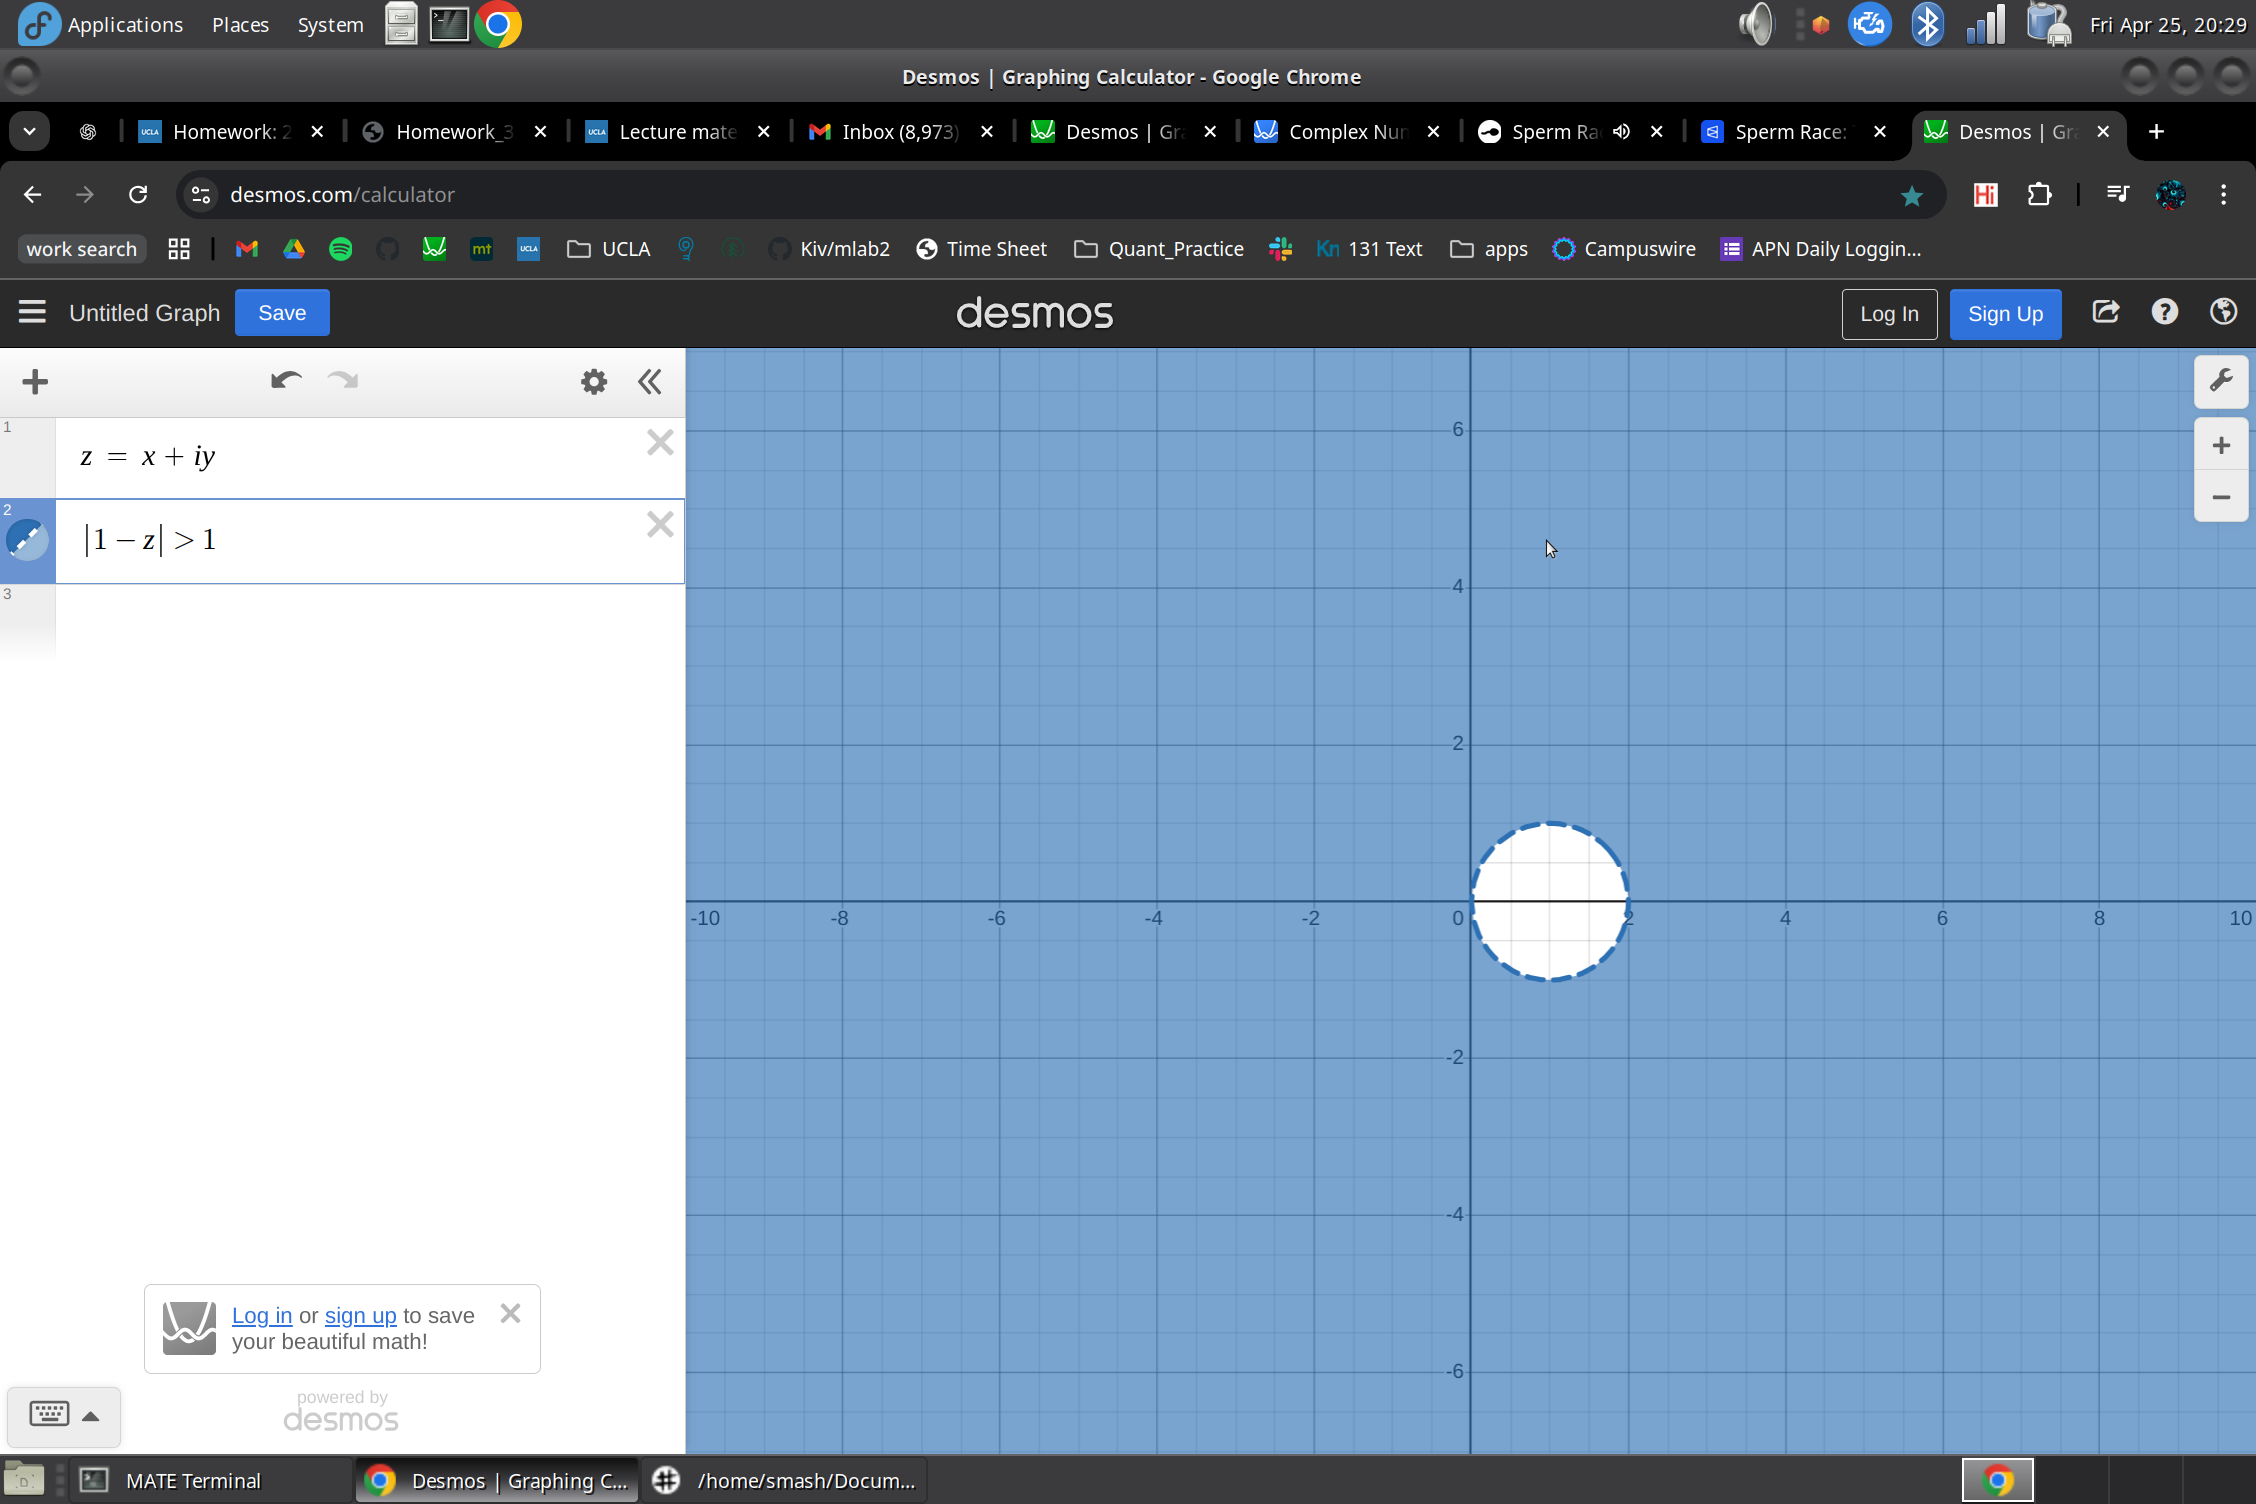
\includegraphics[width=\textwidth]{q1.png}
\item in particular if $\Re(\lambda) < 0$ then for any $h > 0$ we have
    \[
    |1-z| = \sqrt{(1-\Re(\lambda)h)^2 + (\Im(\lambda))^2} \ge 1 - \Re(\lambda)h > 1
    .\] 
    and therefore $|1-z| > 1$ and BE is absolutely stable. for arbitrarily large step size
\item 
    \[
        y' = -100(y-\sin(t)) \hspace{1cm} y(0) = 1
    .\] 
    \begin{enumerate}
        \item Some figures\\
            \includegraphics[width = 10cm]{FE_STEP0.1.png}\\
            \includegraphics[width = 10cm]{FE_STEP0.02.png}\\
            \includegraphics[width = 10cm]{FE_STEP0.01.png}\\
            \includegraphics[width = 10cm]{FE_STEP0.002.png}\\
            using code
            \begin{lstlisting}
import numpy as np
import matplotlib.pyplot as plt

def velocity_field(t, y):
    return -100 * (y- np.sin(t))

# Initial condition
y0 = 1

# Simulation parameters
T = 1
N = 501  # You can adjust this
tvec = np.linspace(0, T, N)
h = tvec[1] - tvec[0]

# Storage for results
y_stored = np.zeros(N)
y_stored[0] = y0
y = y0

for n in range(1,N):
    t = tvec[n]
    y += h * velocity_field(t,y)
    y_stored[n] = y

# Plotting the results

plt.figure(figsize=(8, 6))
plt.plot(tvec, y_stored, 'k-', linewidth=1.5, label='Trajectory')
plt.xlabel('x')
plt.ylabel('y')
plt.title(f'numerical approximation using step size: {h}')
plt.legend()
plt.grid(True)
plt.tight_layout()
plt.savefig(f"FE_Step{h}.png")
plt.show()
 
            \end{lstlisting}
            While step size $h = 0.002$ provides the best solution, $h=0.01$ provides an accurate representation of the trajectory
            whereas $h=0.02$ shows occilation and $h=0.1$ diverges completely.
        \item 
            we can simplify equations and solve directly for $y_{n+1}$ to get
             \[
                 y_{n+1} = \frac{y_n + 100 h \sin(t)}{1 + 100h}
             \]
            \includegraphics[width = 10cm]{BE_STEP0.2.png}\\
            \includegraphics[width = 10cm]{BE_STEP0.1.png}\\
            \includegraphics[width = 10cm]{BE_STEP0.02.png}\\
            \includegraphics[width = 10cm]{BE_STEP0.01.png}\\
            with code
            \begin{lstlisting}
import numpy as np
import matplotlib.pyplot as plt

# Initial condition
y0 = 1

# Simulation parameters
T = 1
N = 101  # You can adjust this
tvec = np.linspace(0, T, N)
h = tvec[1] - tvec[0]

# Storage for results
y_stored = np.zeros(N)
y_stored[0] = y0
y = y0

for n in range(1,N):
    t = tvec[n]
    y = (y+100*h*np.sin(t))/(1 + 100 * h)
    y_stored[n] = y

# Plotting the results

plt.figure(figsize=(8, 6))
plt.plot(tvec, y_stored, 'k-', linewidth=1.5, label='Trajectory')
plt.xlabel('x')
plt.ylabel('y')
plt.title(f'numerical approximation using step size: {h}')
plt.legend()
plt.grid(True)
plt.tight_layout()
plt.savefig(f"BE_Step{h}.png")
plt.show()
            \end{lstlisting}
            here with step size as low as $0.2$ we get a solution that looks approximately like correct solution
            and as $h$ decreases all the way to $0.01$ we get increasingly accurate approximations that all converge.
            It seems that there is no restriction on step size using $BE$ except maybe  $h = 0.3$
    \end{enumerate}
\end{enumerate}        
\end{solution}
\begin{exercise}
\end{exercise}
\begin{solution}
    \begin{enumerate}
        \item  I was excited about the proof that consistency and zero-stability implid convergence for LMMs,
            and I'm excited to learn more about when to apply different numerical integrators.
        \item I find it challenging to memorize all of the methods and concepts in the class and I find myself
            referring to my notes often to answer questions, which I will have to counterbalance for the midterm.
    \end{enumerate}
\end{solution}

\end{document}

